\documentclass[fleqn,10pt]{article}
\usepackage[a4paper, margin=1.0in]{geometry}
\usepackage{listings}
\usepackage{lstlhs}
\usepackage{xcolor}
\usepackage{graphicx}
\def\includepicture#1{\includegraphics{#1.eps}}
\usepackage{hyperref}
\usepackage{threadq}

\parindent=0pt % I hate first line indentation
\parskip=3pt   % I like a visual white gap between paragraphs


\title{RTEMS Thread Queue Simulation}
\author{Andrew Butterfield}
\date{\today}

\begin{document}

\maketitle
\tableofcontents


\bibliographystyle{alpha}

\newpage\section{Introduction}

This document provides simulations of the various thread queue designs used
in the RTEMS operating system. 
These range from simple first-in first-out (FIFO) designs,
through priority-based approaches, 
to algorithms for SMP that support schedulability analysis.

We focus on thread queues for RTEMS Tasks waiting to gain access
to a shared resource, via a mutex lock.

The basic building blocks are a simple FIFO queue, 
and a priority queue that assumes all threads have a unique priority.

The most complex form is a round-robin/FIFO queue 
whose contents are priority queues, 
one for each scheduling cluster.
This is used to implement the 
Multiprocessor Resource Sharing Protocol(MrsP) 
thread queue algorithm.


Key papers are: 
\cite{Burns:2013:MrsP}, 
\cite{Brandenburg:2013:OMIP},
\cite{Catellani:2015:MrsP},
\cite{Garrido:2017:MrsP},
\cite{Zhao:2017:MrsP},
\cite{Gomes:2019:MrsP},
\cite{Zhao:2020:MrsP},
\cite{Zhao:2021:MrsP}
.

Most relevent RTEMS documents:
\cite{RTEMS:CUSER}, 
\cite{RTEMS:ENG}, 
and \cite{RTEMS:USERM}.

% What about \cite{RTEMS:Classic} ?
\newpage\input{src/Queues.lhs}
\newpage\input{src/SimState.lhs}
\newpage\input{src/Runner.lhs}
\newpage\input{app/Main.lhs}
\newpage\input{test/Spec.lhs}

\newpage
\bibliography{MAIN}

\appendix

\newpage\section{Notes}

\begin{itemize}
    \item  Read Thread Queues \cite[\S3.5]{RTEMS:CUSER}
      (\url{https://docs.rtems.org/branches/master/c-user/key_concepts.html#thread-queues})
    \item 
      ``priority-based, preemptive algorithm augmented to provide round-robin
        characteristics within individual priority groups. The goal \dots is to
        guarantee that the task which is executing on the processor at any point
        in time is the one with the highest priority among all tasks in the
        ready state.''
        \cite[\S5.2.2]{RTEMS:CUSER}
    \item 
      ``Another mechanism is to maintain a list of FIFOs per priority. 
        When a task is readied, 
        it is placed on the rear of the FIFO for its priority.
        This method is often used with a bitmap to assist in
        locating which FIFOs have ready tasks on them. 
        This data structure has $O(1)$ insert, extract and 
        find highest ready run-time complexities.''
        \cite[\S5.2.2]{RTEMS:CUSER}
    \item 
      ``RTEMS provides four mechanisms which allow the user to alter 
        the task scheduling decisions:
        \begin{itemize}
            \item user-selectable task priority level
            \item task preemption control
            \item task timeslicing control
            \item manual round-robin selection
    \end{itemize}''
      \cite[\S5.2.3]{RTEMS:CUSER}
    \item 
      ``The evaluation order for scheduling characteristics is always priority,
        preemption mode, and timeslicing. 
        When reading the descriptions of timeslicing and manual round-robin
        it is important to keep in mind that preemption (if enabled)
        of a task by higher priority tasks will occur as required, 
        overriding the other factors presented in the description.''
        \cite[\S5.2.3]{RTEMS:CUSER}
    \item 
      ``Note that the preemption setting has no effect on the manner
        in which a task is scheduled. 
        It only applies once a task has control of the processor.''
        \cite[\S5.2.3.2]{RTEMS:CUSER}
    \item
      Task State Transitions \cite[\S5.2.5]{RTEMS:CUSER}
      \\
      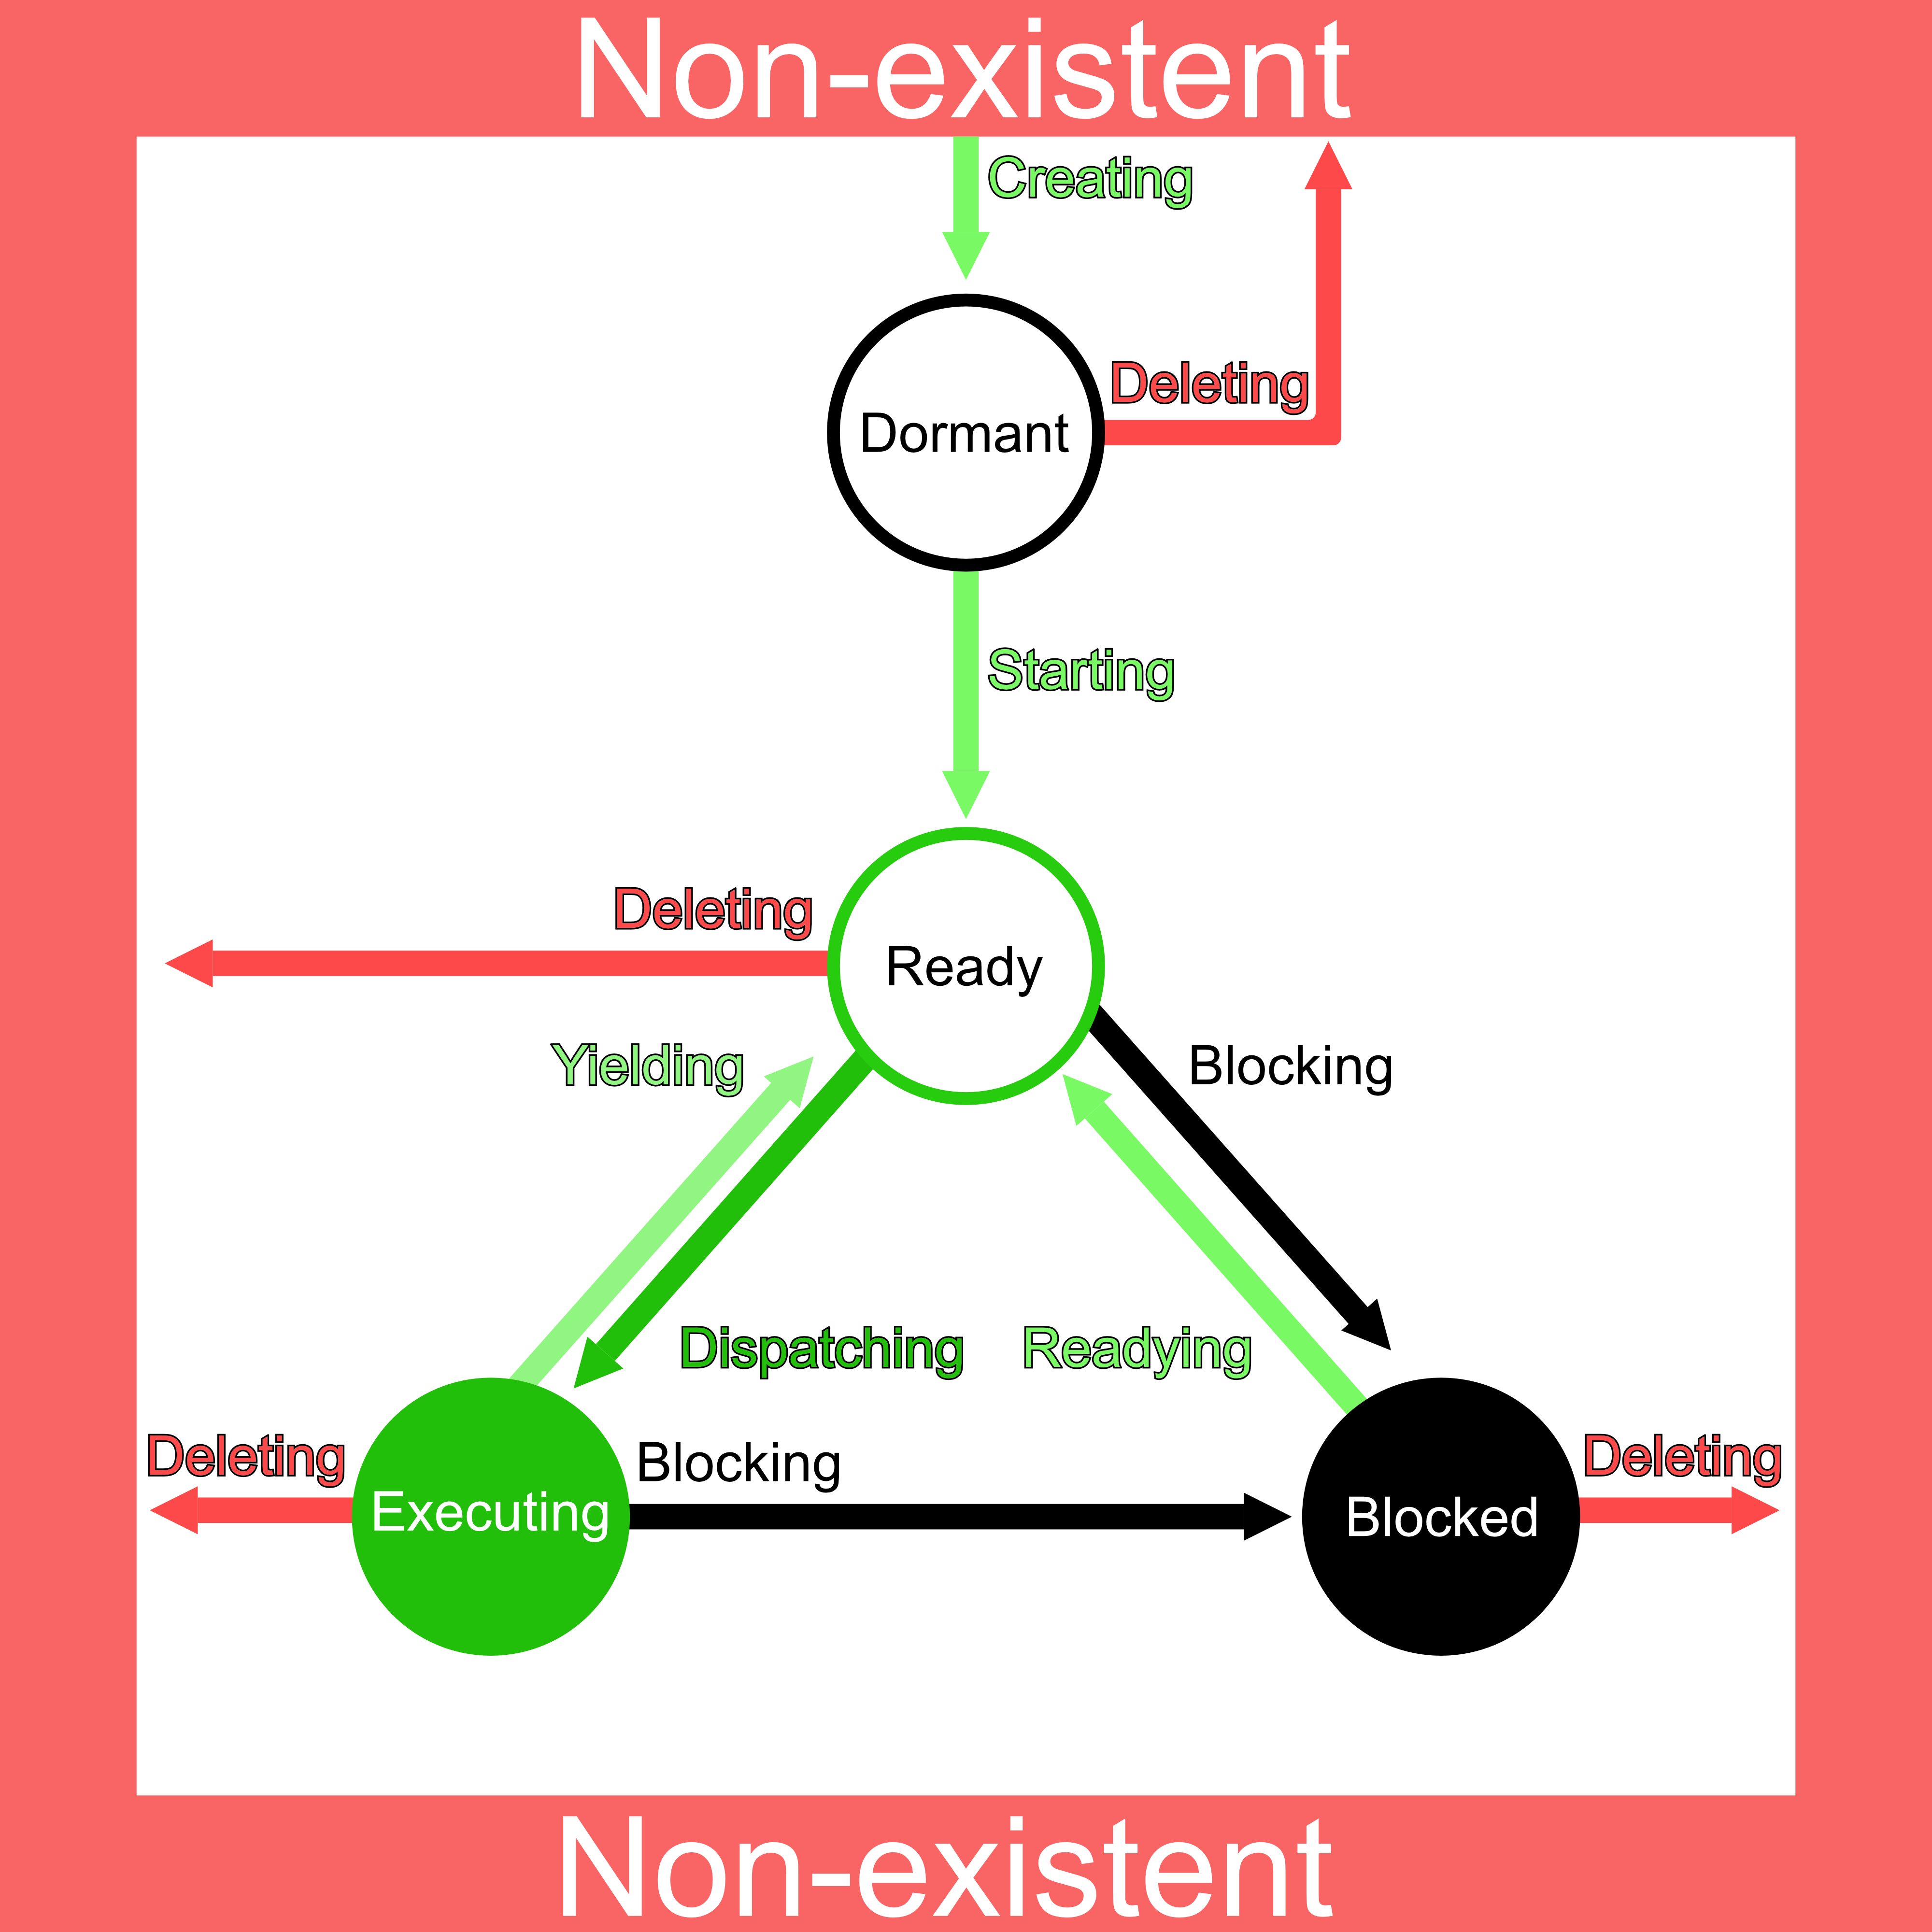
\includegraphics[scale=0.3]{images/states.png}
    \item
      ``All SMP schedulers included in RTEMS are priority based. 
       The processors managed by a scheduler instance are allocated 
       to the highest priority tasks allowed to run.``
      \cite[\S5.4]{RTEMS:CUSER}
    \item 
      The Earliest Deadline First SMP Scheduler is the default in SMP configurations
      if more than one processor is configured
      \cite[\S5.4.1]{RTEMS:CUSER}
      (\url{https://docs.rtems.org/branches/master/c-user/scheduling-concepts/smp-schedulers.html})
    \item TODO: SMP
      (\url{https://docs.rtems.org/branches/master/c-user/symmetric_multiprocessing_services.html})
\end{itemize}





\end{document}
